% DO NOT COMPILE THIS FILE DIRECTLY!
% This is included by the other .tex files.

\begin{frame}[t,plain]
\titlepage
\end{frame}

\begin{frame}[t]{Temática}

\begin{figure}[!h]
    \centering
    
\includegraphics[scale=1.35]{fbig.png}
    \label{fig:my_label}
\end{figure}

\end{frame}






\begin{frame}[t,fragile]{Licencias y Softwares Asociados}
Los software y licencias asociadas a la aplicación son los siguientes:
AFNetworking, Appirater, Boost, CocoaLumberjack, Cocoawithlove, Flick-OAuth-iOS
    ,Google Breakpad entre muchos otros
\bigskip


De los cuales se hace una subdivisión por:

\begin{itemize}
    \item Creación de Servicios (Android y iOS)
    \item Conexión a Servidores (Android y iOS)
    \item Aplicaciones Propias de dispositivos (Android y iOS)
\end{itemize}



\end{frame}


\begin{frame}[t,fragile]{Propuesta de Problemas}
Además de las herramientas utilizadas se consideran realizar las siguientes pruebas:

\begin{itemize}
    \item Validar la Seguridad de la Aplicación en Base a sus Herramientas/Software.
    \item Analizar el React Native de Instagram para Andriod y iOS.
    \item Realizar Pruebas Asociadas a la conexión Servidor Aplicación. haciendo uso de:
    \begin{itemize}
        \item Man-in-the-middle.
        \item DDoS.
    \end{itemize}
    \item Decompilar la Aplicación (si es posible).
    \item  Analizar ataque por medio de Restauración de Contraseña haciendo uso de Proxy Web. (ataque 2016).
    \item Posible Descompilación del Código.
    
    
\end{itemize}



\end{frame}

\begin{frame}[t,fragile]{Data de Problemas Relevantes}

\textbf{Vulnerabilidad en OAuth 2013}


\begin{wrapfigure}{l}{0.43\textwidth} 
\vspace{2pt}
  \begin{center}
    
\includegraphics[width=0.4\textwidth]{oauth}
    \label{fig:databaseUserTable}
  \end{center}
  \vspace{2pt}
\end{wrapfigure} 

\bigskip

Luego de la compra de Facebook , se logra encontrar una falla de seguridad del software relacionada a la privacidad y confidencialidad de los datos, utilizando el protocolo OAuth. Dicho problema abrió paso a problemas como el acceso a la lista de amigos en Fb o filtración de imgenes.




\end{frame}

\begin{frame}[t,fragile]{Data de Problemas Relevantes}

\textbf{Cuentas Compartidas 2016}


\begin{wrapfigure}{r}{0.43\textwidth} 
\vspace{2pt}
  \begin{center}
    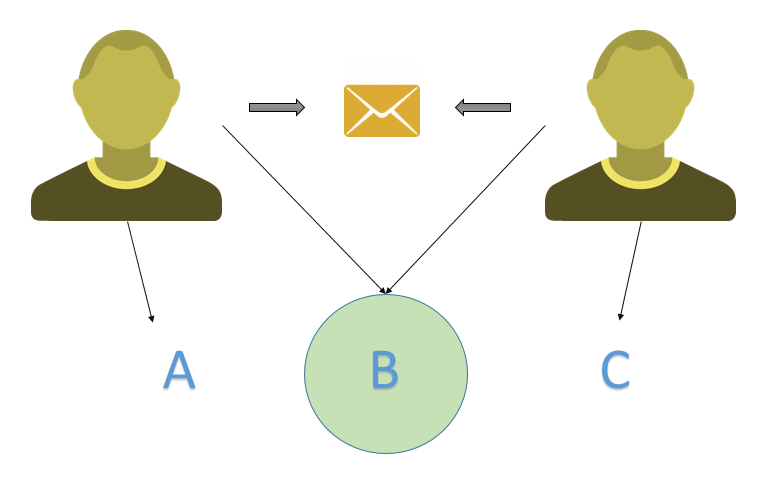
\includegraphics[width=0.5\textwidth]{compartidaig.png}
    \label{fig:databaseUserTable}
  \end{center}
  \vspace{2pt}
\end{wrapfigure} 

\bigskip

Consiste en la compartición de cuentas por parte de un Sujeto 1 v's un Sujeto 2, donde ambos ya sea por motivos de asociación u otros comparten una cuenta en común B, dando paso a la notificación de cuentas fuera de su alcance. Lo que implica una filtración de información fuera del consentimiento de cada sujeto.

\end{frame}


\begin{frame}[t,fragile]{Data de Problemas Relevantes}

\textbf{Hackeo de Cuentas 2017}


\begin{wrapfigure}{l}{0.43\textwidth} 
\vspace{2pt}
  \begin{center}
    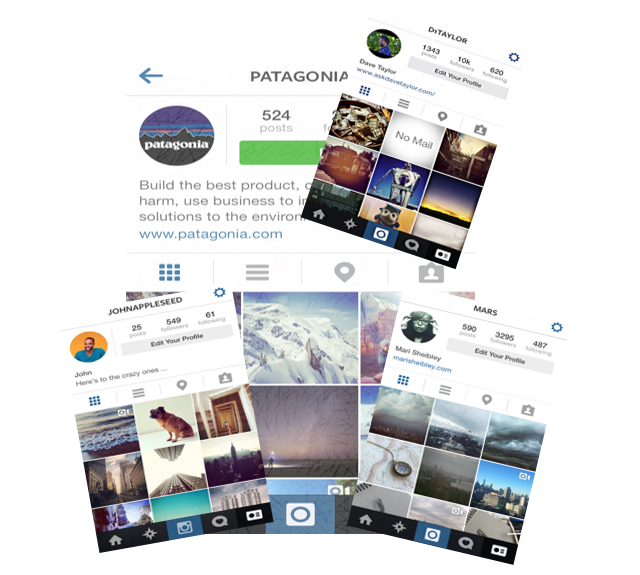
\includegraphics[width=0.45\textwidth]{accounts.png}
    \label{fig:databaseUserTable}
  \end{center}
  \vspace{2pt}
\end{wrapfigure} 

\bigskip

Hackeo masivo de cuentas, comprometiendo la seguridad de las cuentas en redes sociales. Llegando a circular datos de acceso a los perfiles a \$10 dolares cada cuenta. La información fue almacenada en la base de datos \textbf{Doxagram} en donde se realizó la venta.



\end{frame}

\begin{frame}[t,fragile]{Descarga de Aplicación}

\textbf{Obtención de Apk}


\begin{figure}[!h]
    \centering
    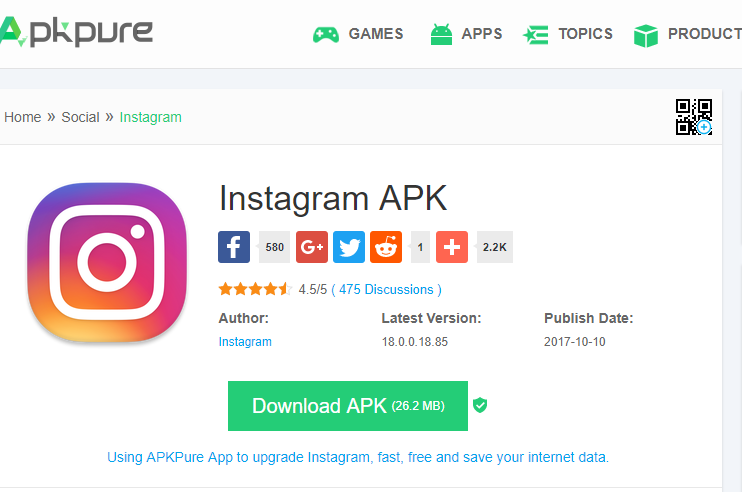
\includegraphics[scale=0.4]{apkpure.png}
    \label{fig:my_label}
\end{figure}

\end{frame}

\begin{frame}[t,fragile]{Decompilación}

\textbf{Obtención de Archivos}


\begin{wrapfigure}{r}{0.43\textwidth} 
\vspace{2pt}
  \begin{center}
    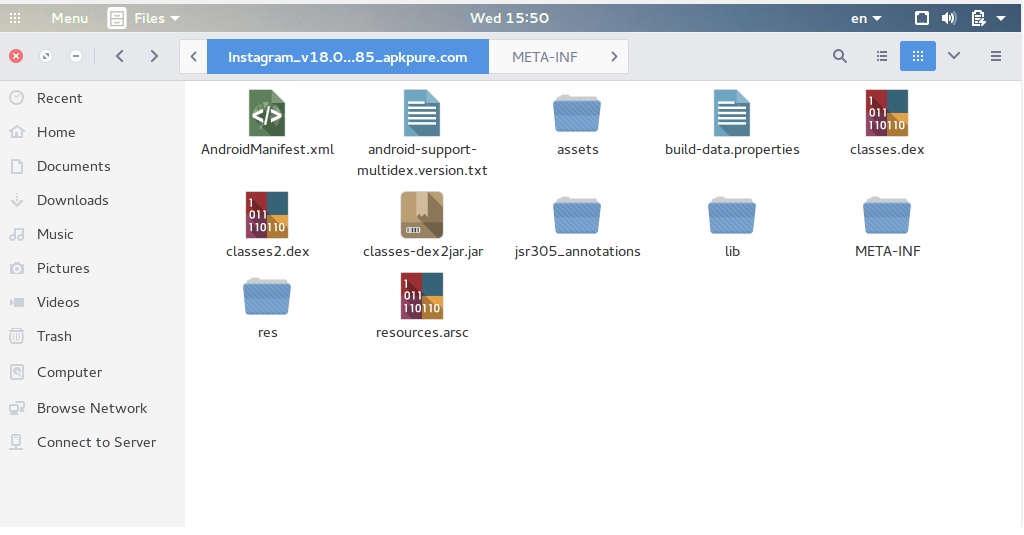
\includegraphics[width=0.45\textwidth]{decompiladaapk.png}
    \label{fig:databaseUserTable}
  \end{center}
  \vspace{2pt}
\end{wrapfigure} 

\bigskip

Tras descargar el apk de instagram se utiliza la siguiente metodología:

\begin{itemize}
    \item Convertir archivo a .ZIP, para obtener archivos.
    \item Obtención de XML, classes.dex, lib y Meta-inf.
\end{itemize}


\end{frame}




\begin{frame}[t,fragile]{Decompilación}

\textbf{META-INF}


\begin{wrapfigure}{r}{0.43\textwidth} 
\vspace{2pt}
  \begin{center}
    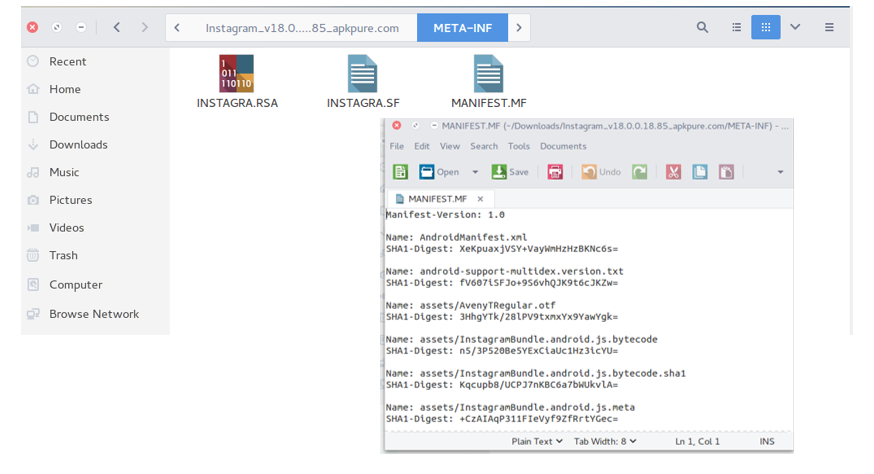
\includegraphics[width=0.45\textwidth]{meta-inf2.png}
    \label{fig:databaseUserTable}
  \end{center}
  \vspace{2pt}
\end{wrapfigure} 

\bigskip

En ésta carpeta es posible encontrar los métodos utilizados en la aplicación para la realización de encriptación y seguridad propiamente tal de los archivos dentro del desarrollo. Destacando entonces herramientas como:

\begin{itemize}
    \item RSA (cifrado)
    \item SHA1 (hashing)
\end{itemize}


\end{frame}




\begin{frame}[t,fragile]{Decompilación}

\textbf{Uso de Apktool}

\begin{wrapfigure}{r}{0.43\textwidth} 
\vspace{2pt}
  \begin{center}
    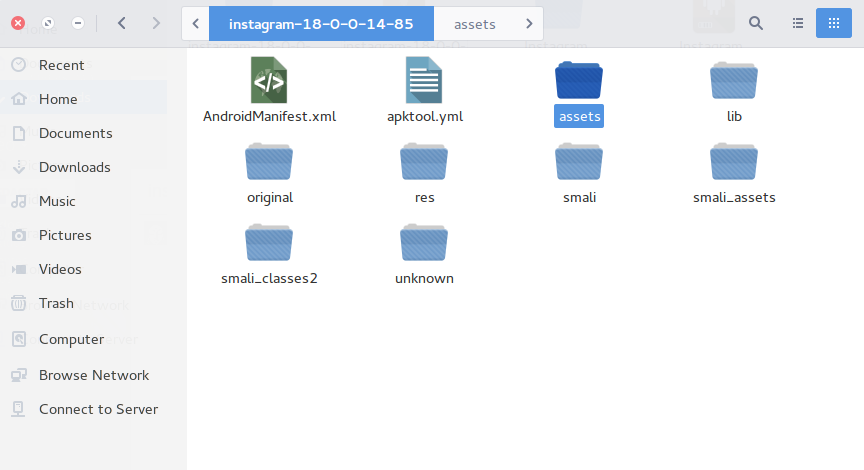
\includegraphics[width=0.45\textwidth]{apktool.png}
    \label{fig:databaseUserTable}
  \end{center}
  \vspace{2pt}
\end{wrapfigure} 

\bigskip

Uso de herramienta \textbf{apktool} 
\begin{center}
    apktool d Instagram.apk
\end{center}
 \\
 
 se obtendrá archivos correspondientes a la aplicación además de los layouts, res y clasess especificas del mismo.

\end{frame}

\begin{frame}[t,fragile]{Decompilación}

\textbf{Obtención de XML}

\begin{wrapfigure}{r}{0.43\textwidth} 
\vspace{2pt}
  \begin{center}
    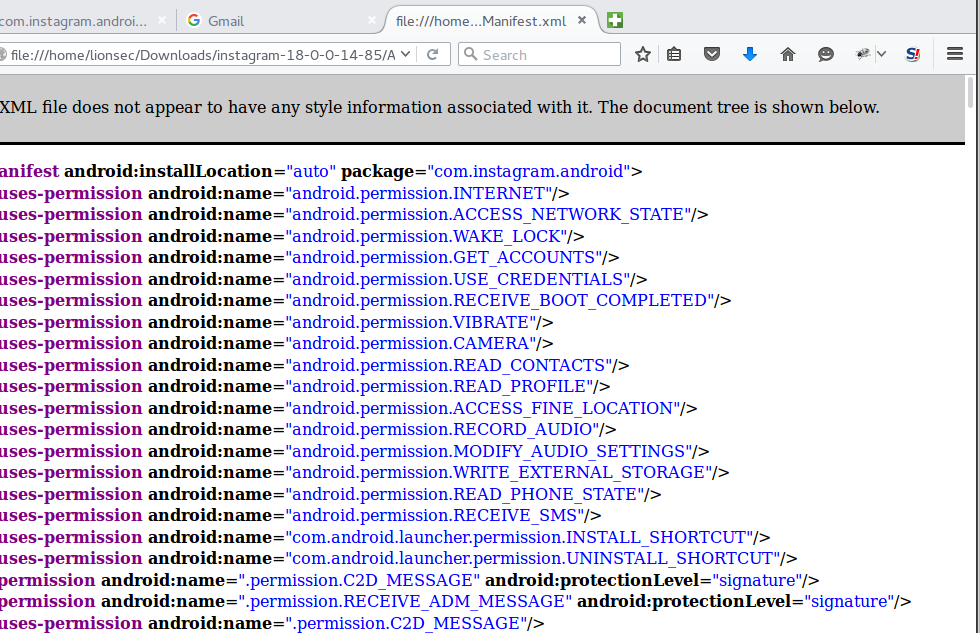
\includegraphics[width=0.45\textwidth]{xml.png}
    \label{fig:databaseUserTable}
  \end{center}
  \vspace{2pt}
\end{wrapfigure} 

\bigskip

 Por medio de la herrramienta \textbf{apktool} y utilizando consola. se aplica comando
\begin{center}
    apktool d Instagram.apk
\end{center}
 \\
 
 se obtendrá los xml y archivos correspondientes a la aplicación.

\end{frame}

\begin{frame}[t,fragile]{Decompilación}

\textbf{Obtención de Java}

\begin{wrapfigure}{r}{0.43\textwidth} 
\vspace{2pt}
  \begin{center}
    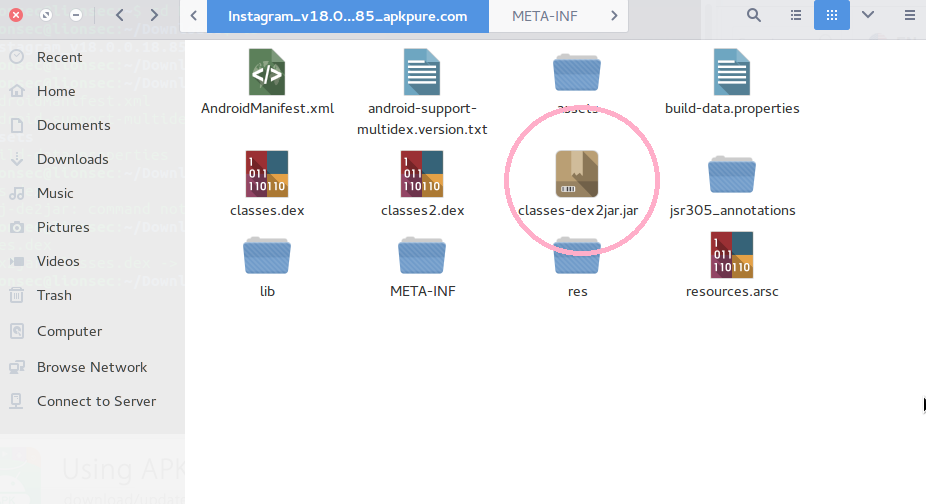
\includegraphics[width=0.45\textwidth]{jarclases.png}
    \label{fig:databaseUserTable}
  \end{center}
  \vspace{2pt}
\end{wrapfigure} 

\bigskip

 Por medio de la herramienta \textbf{dex2jar} y utilizando consola. se aplica comando
\begin{center}
    d2j-dex2jar classes.dex
\end{center}
 \\
 
 se utiliza el dex (Dalvik Executable) para obtener el comprimido del archivo APK. Lo que puede ser visto con un java decompiler, accediendo entonces a el archivo.

\end{frame}


\begin{frame}[t,fragile]{Decompilación}

\textbf{Ver Archivos React}

\begin{wrapfigure}{r}{0.43\textwidth} 
\vspace{2pt}
  \begin{center}
    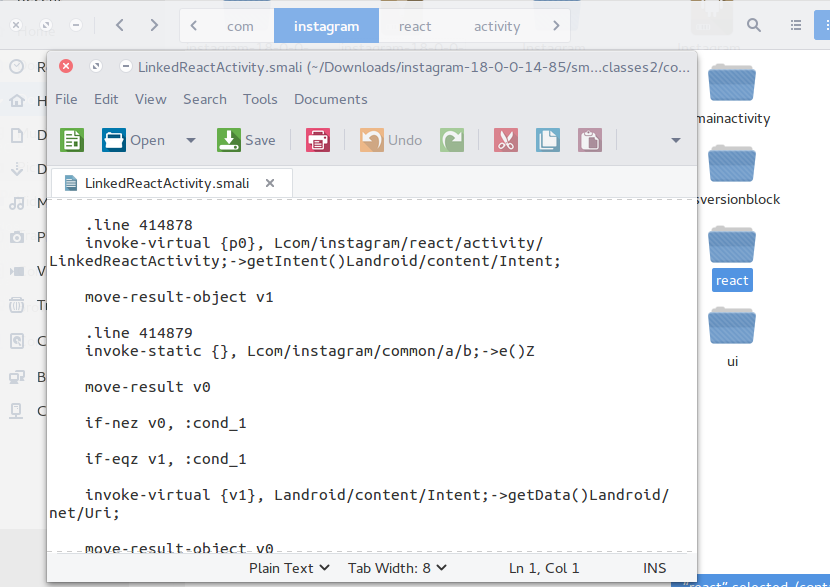
\includegraphics[width=0.45\textwidth]{react.png}
    \label{fig:databaseUserTable}
  \end{center}
  \vspace{2pt}
\end{wrapfigure} 

\bigskip

 Se encuentran los archivos de react correspondiente las actividades, delegados o bien los archivos \textbf{.smali} correspondientes al assembly de lenguaje Java.

\end{frame}